% This is part of Un soupçon de mathématique sans être agressif pour autant
% Copyright (c) 2015
%   Laurent Claessens
% See the file fdl-1.3.txt for copying conditions.

{\Large Cette activité ne va pas. Il faut trouver un graphique plus simple.}

%--------------------------------------------------------------------------------------------------------------------------- 
\subsection*{Activité : placer dans un repère}
%---------------------------------------------------------------------------------------------------------------------------

Répondre aux questions en se servant du graphique :

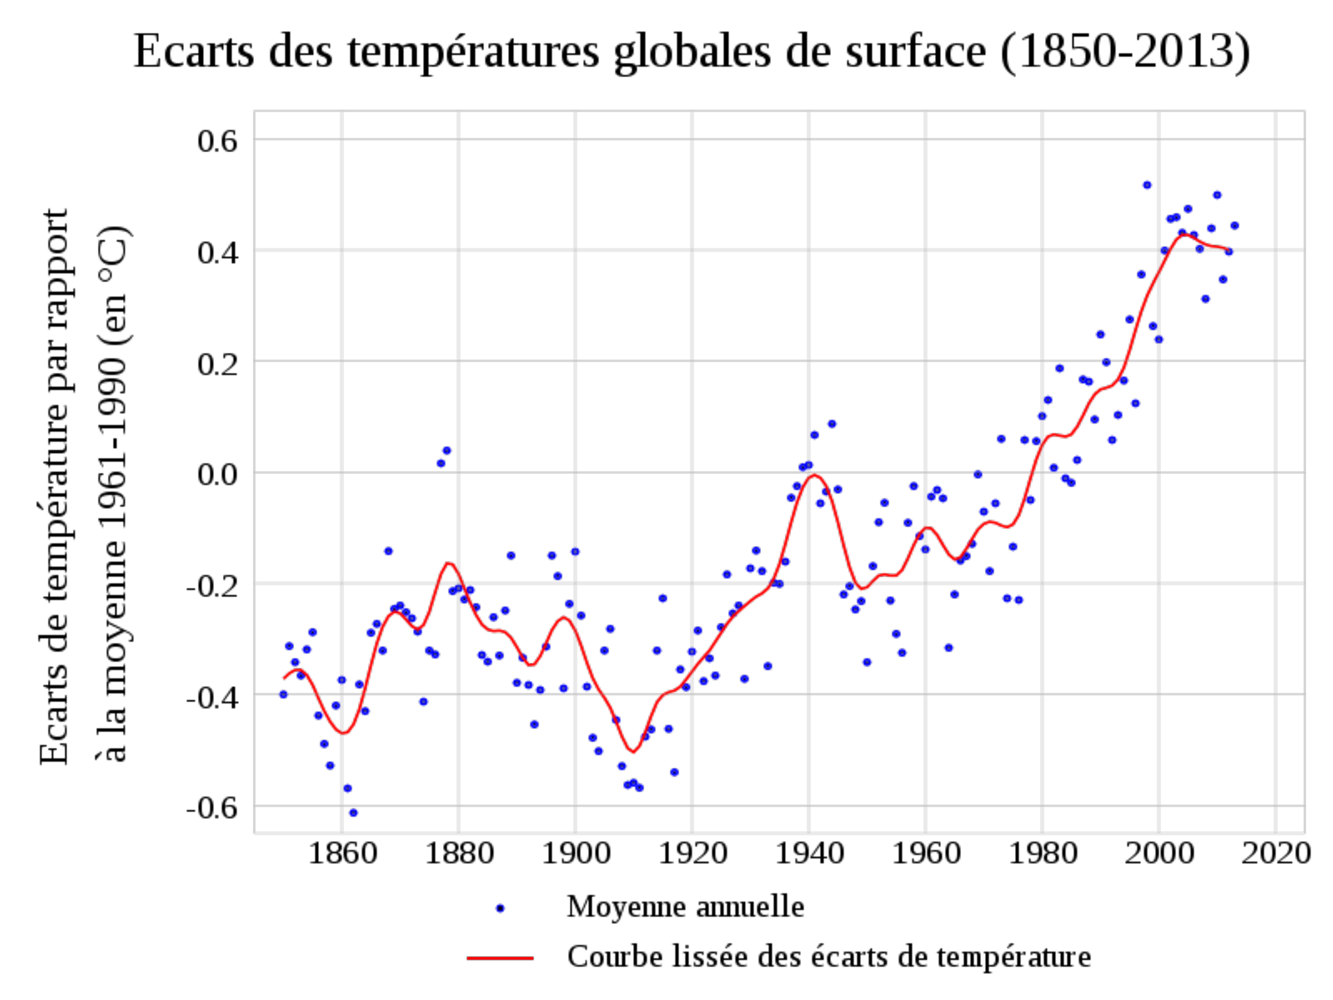
\includegraphics[width=0.7\textwidth]{EcartsTempSurface2013.pdf}

De \url{http://fr.wikipedia.org/wiki/Réchauffement_climatique}


\begin{enumerate}
    \item
        Entre \( 1900\) et \( 1910\), on observe une belle dégringolade. De combien de degré environ ?
    \item
        Quel est l'écart de température entre l'année la plus chaude et la plus froide enregistrée ?
    \item
        Quelle est l'écart de température entre l'année \( 1980\) et \( 1920\) ?
    \item
        Donner quelques années pour lesquelles la température ont été (environ) dans la moyenne \( 1961-1990\).
\end{enumerate}
